\begin{landscape}

\section{Arbeitsablaufplan}
\begin{center}
\begin{tabular}{ll|r|r|}
\hline
\multicolumn{1}{|c|}{Pos.} & Arbeitsschritt & ~~Soll~~ & ~~Ist~~ \\ \hline
\multicolumn{1}{|c|}{1} & Informationsphase & 2,0h & 2,0h \\ \hline
\multicolumn{1}{|c|}{2} & Planungsphase & 1,0h & 1,0h \\ \hline
\multicolumn{1}{|c|}{3} & Anfertigung eines Arbeitsablaufplans & 1,0h & 1,0h \\ \hline
\multicolumn{1}{|c|}{4} & Schreiben eines Lastenheftes für die Herstellung des Signalgenerators & 2,5h & 2,5h \\ \hline
\multicolumn{1}{|c|}{5} & Anfertigung eines Inbetriebnahmeprotokolls für den Signalgenerator & 2,5h & 3,0h \\ \hline
\multicolumn{1}{|c|}{6} & Schreiben eines Lastenheftes für die Herstellung des Gehäuses & 2,0h & 1,0h \\ \hline
\multicolumn{1}{|c|}{7} & Anfertigung eines Übergabeprotokolls für das Gehäuse und Signalgenerator & 1,0h & 1,0h \\ \hline
\multicolumn{1}{|c|}{8} & Ausfüllen des Inbetriebnahmeprotokolls für den Signalgenerator & 1,0h & 1,0h \\ \hline
\multicolumn{1}{|c|}{9} & Ausfüllen des Übergabeprotokolls des Gehäuses & 0,5h & 0,5h \\ \hline
\multicolumn{1}{|c|}{10} & Montage des Signalgenerators in das Gehäuse & 0.5h & 1,0h \\ \hline
\multicolumn{1}{|c|}{11} & Aufstellen einer Kostenübersicht des Projektes & 2,0h & 2,5h \\ \hline
\multicolumn{1}{|c|}{12} & Kontrollphase & 4,0h & 4,0h \\ \hline
                       &  & 20,0h & 20,5h \\ \cline{3-4} 
\end{tabular}
\end{center}
\pagebreak
\subsection{Zeitlicher Verlauf der Arbeiten}
\begin{center}
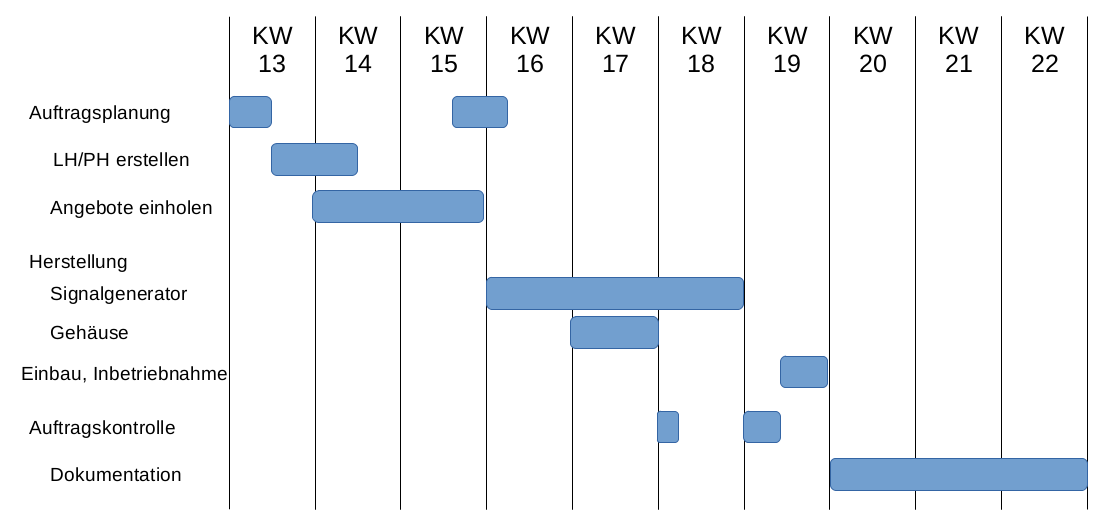
\includegraphics[width=1.4\textwidth]{./img/zeitstrahl.png}
\end{center}
\end{landscape}
